\documentclass{article}
\usepackage[utf8]{inputenc}
\usepackage[english]{babel}
\usepackage[table]{xcolor}
\usepackage{siunitx}
\usepackage{geometry}
\usepackage{graphicx}
\usepackage{longtable}
\usepackage{booktabs}
\usepackage{amsmath}
\usepackage{amssymb}
\usepackage{array}
\geometry{
  left=0.5in,
  top=0.2in,
  right=0.5in,
  bottom=0.5in
}
\sisetup{
  round-mode=places, % Rounds numbers
  round-precision=2, % to 2 places
}
\definecolor{B}{HTML}{6495ed} % cornflowerblue
\definecolor{G}{HTML}{20b2aa} % lightseagreen
\def\DA#1{\textcolor{B}{\textbf{#1}}}
\def\DB#1{\textcolor{G}{\textbf{#1}}}
\def\A#1{\textbf{#1}}
\def\B#1#2#3{\hspace*{#2}\textbf{#1}\hspace*{#3}}
\graphicspath{{./images/}} % image path
\title{Analysis of C. elegans on Drugs Lab Report}
\author{Philip Kim}
\date{\today}
\begin{document}
\maketitle
\vspace*{-1cm}
\begin{center}
  \begin{longtable}[c]{|c|r|r|r|}
    \toprule
    \textbf{\textcolor{white}{\#}} &
    \A{\textcolor{white}{Drug A -\ Control A}} &
    \A{\textcolor{white}{Drug A -\ Control A}} &
    \A{\textcolor{white}{Drug A -\ Control A}}\\
    \textbf{\#} &
    \B{Drug \DA{A}}{0em}{3em} &
    \B{Control \DA{A}}{0em}{2em} &
    \B{Drug \DA{A} -\ Control \DA{A}}{0em}{0em}\\
    \textbf{\textcolor{white}{\#}} &
    \textbf{\textcolor{white}{\#}} &
    \textbf{\textcolor{white}{\#}} &
    \textbf{\textcolor{white}{\#}}\\
    \midrule\endfirsthead%
    \toprule
    \textbf{\textcolor{white}{\#}} &
    \A{\textcolor{white}{Drug A -\ Control A}} &
    \A{\textcolor{white}{Drug A -\ Control A}} &
    \A{\textcolor{white}{Drug A -\ Control A}}\\
    \textbf{\#} &
    \B{Drug A}{0em}{3em} &
    \B{Control A}{0em}{2em} &
    \B{Drug A -\ Control A}{0em}{0em}\\
    \textbf{\textcolor{white}{\#}} &
    \textbf{\textcolor{white}{\#}} &
    \textbf{\textcolor{white}{\#}} &
    \textbf{\textcolor{white}{\#}}\\
    \midrule\endhead%
      1 & 40.20 & 22.40 & 17.80\\\midrule
      2 & 7.60 & 9.90 & -2.30\\\midrule
      3 & 0.00 & 6.20 & -6.20\\\midrule
      4 & 15.10 & 18.10 & -3.00\\\midrule
      5 & 10.50 & 20.50 & -10.00\\\midrule
      6 & 5.50 & 2.00 & 3.50\\\midrule
      7 & 22.50 & 25.00 & -2.50\\\midrule
      8 & 12.60 & 23.30 & -10.70\\\midrule
      9 & 3.00 & 15.00 & -12.00\\\midrule
      10 & 0.00 & 11.00 & -11.00\\
    \bottomrule
  \end{longtable}
  % Drug A Effect:
  %   mean: -3.64
  %   stddev: 9.04
  %   n: 10
  %   stderr: 2.86
  %   2*stderr: 5.72 (95% ci)
  %   mean+2*stderr: 2.08 (upper ci)
  %   mean-2*stderr: -9.36 (lower ci)
  % Drug A Graph:
  %   mean: -3.64
  %   2*stderr: 5.72 (95% ci)
  %   ci overlaps with 0, therefore drug a has no significant difference on C. elegans
  \begin{center}
    \subsection*{Drug \DA{A} Effect:}
    \begin{align*}
      N&= 10 \\
      \overline{\DA{A}}&=\tfrac{\DA{A}_1 + \DA{A}_2 + \cdots + \DA{A}_N}{N}\\
      &=\boxed{ - 3.64}\\
      \sigma_{\DA{A}}&= \sqrt{\tfrac{\left|\DA{A}_1 - \overline{\DA{A}}\right|^2 + \cdots + \left|\DA{A}_N - \overline{\DA{A}}\right|^2}{N - 1}}\\
      &=\boxed{9.04}\\
      \epsilon_{\DA{A}}&= \tfrac{\sigma_{\DA{A}}}{\sqrt{N}}\\
      &=\boxed{2.86}\\
      \mathcal{CI}_{\DA{A}}&= 2\times \epsilon_{\DA{A}}\\
      &=\boxed{5.72~(95\%~\mathcal{CI}_{\DA{A}})}\\
      Upper~\mathcal{CL}_{\DA{A}}&=\overline{\DA{A}} +\left(\mathcal{CI}_{\DA{A}}\right)\\
      &=\boxed{2.08}\\
      Lower~\mathcal{CL}_{\DA{A}}&=\overline{\DA{A}} -\left(\mathcal{CI}_{\DA{A}}\right)\\
      &=\boxed{ - 9.36}\\
    \end{align*}
  \end{center}
  \newpage
  \begin{longtable}[c]{|c|r|r|r|}
    \toprule
    \textbf{\textcolor{white}{\#}} &
    \A{\textcolor{white}{Drug B -\ Control B}} &
    \A{\textcolor{white}{Drug B -\ Control B}} &
    \A{\textcolor{white}{Drug v -\ Control B}}\\
    \textbf{\#} &
    \B{Drug \DB{B}}{0em}{3em} &
    \B{Control \DB{B}}{0em}{2em} &
    \B{Drug \DB{B} -\ Control \DB{B}}{0em}{0em}\\
    \textbf{\textcolor{white}{\#}} &
    \textbf{\textcolor{white}{\#}} &
    \textbf{\textcolor{white}{\#}} &
    \textbf{\textcolor{white}{\#}}\\
    \midrule\endfirsthead%
    \toprule
    \textbf{\textcolor{white}{\#}} &
    \A{\textcolor{white}{Drug B -\ Control B}} &
    \A{\textcolor{white}{Drug B -\ Control B}} &
    \A{\textcolor{white}{Drug B -\ Control B}}\\
    \textbf{\#} &
    \B{Drug B}{0em}{3em} &
    \B{Control B}{0em}{2em} &
    \B{Drug B -\ Control B}{0em}{0em}\\
    \textbf{\textcolor{white}{\#}} &
    \textbf{\textcolor{white}{\#}} &
    \textbf{\textcolor{white}{\#}} &
    \textbf{\textcolor{white}{\#}}\\
    \midrule\endhead%
      1 & 33.70 & 26.30 & 7.40\\\midrule
      2 & 18.90 & 8.00 & 10.90\\\midrule
      3 & 15.00 & 9.00 & 6.00\\\midrule
      4 & 19.40 & 20.60 & -1.20\\\midrule
      5 & 41.20 & 13.57 & 27.63\\\midrule
      6 & 49.80 & 18.50 & 31.30\\\midrule
      7 & 36.10 & 21.90 & 14.20\\\midrule
      8 & 28.50 & 24.90 & 3.60\\\midrule
      9 & 23.90 & 22.10 & 1.80\\\midrule
      10 & 35.50 & 16.90 & 18.60\\
    \bottomrule
  \end{longtable}
  % Drug B Effect:
  %   mean: 12.04
  %   stddev: 10.92
  %   n: 10
  %   stderr: 3.45
  %   2*stderr: 6.90 (95% ci)
  %   mean+2*stderr: 18.83 (upper ci)
  %   mean-2*stderr: 5.12 (lower ci)
  % Drug B Graph:
  %   mean: 12.02
  %   2*stderr: 6.90 (95% ci)
  %   ci does not overlaps with 0, therefore drug b has a positive significant difference on C. elegans
  \begin{center}
    \subsection*{Drug \DB{B} Effect:}
    \begin{align*}
      N&= 10 \\
      \overline{\DB{B}}&=\tfrac{\DB{B}_1 + \DB{B}_2 + \cdots + \DB{B}_N}{N}\\
      &=\boxed{12.04}\\
      \sigma_{\DB{B}}&= \sqrt{\tfrac{\left|\DB{B}_1 - \overline{\DB{B}}\right|^2 + \cdots + \left|\DB{B}_N - \overline{\DB{B}}\right|^2}{N - 1}}\\
      &=\boxed{10.92}\\
      \epsilon_{\DB{B}}&= \tfrac{\sigma_{\DB{B}}}{\sqrt{N}}\\
      &=\boxed{3.45}\\
      \mathcal{CI}_{\DB{B}}&= 2\times \epsilon_{\DB{B}}\\
      &=\boxed{6.90~(95\%~\mathcal{CI}_{\DB{B}})}\\
      Upper~\mathcal{CL}_{\DB{B}}&=\overline{\DB{B}} +\left(\mathcal{CI}_{\DB{B}}\right)\\
      &=\boxed{18.83}\\
      Lower~\mathcal{CL}_{\DB{B}}&=\overline{\DB{B}} -\left(\mathcal{CI}_{\DB{B}}\right)\\
      &=\boxed{5.12}\\
    \end{align*}
  \end{center}
  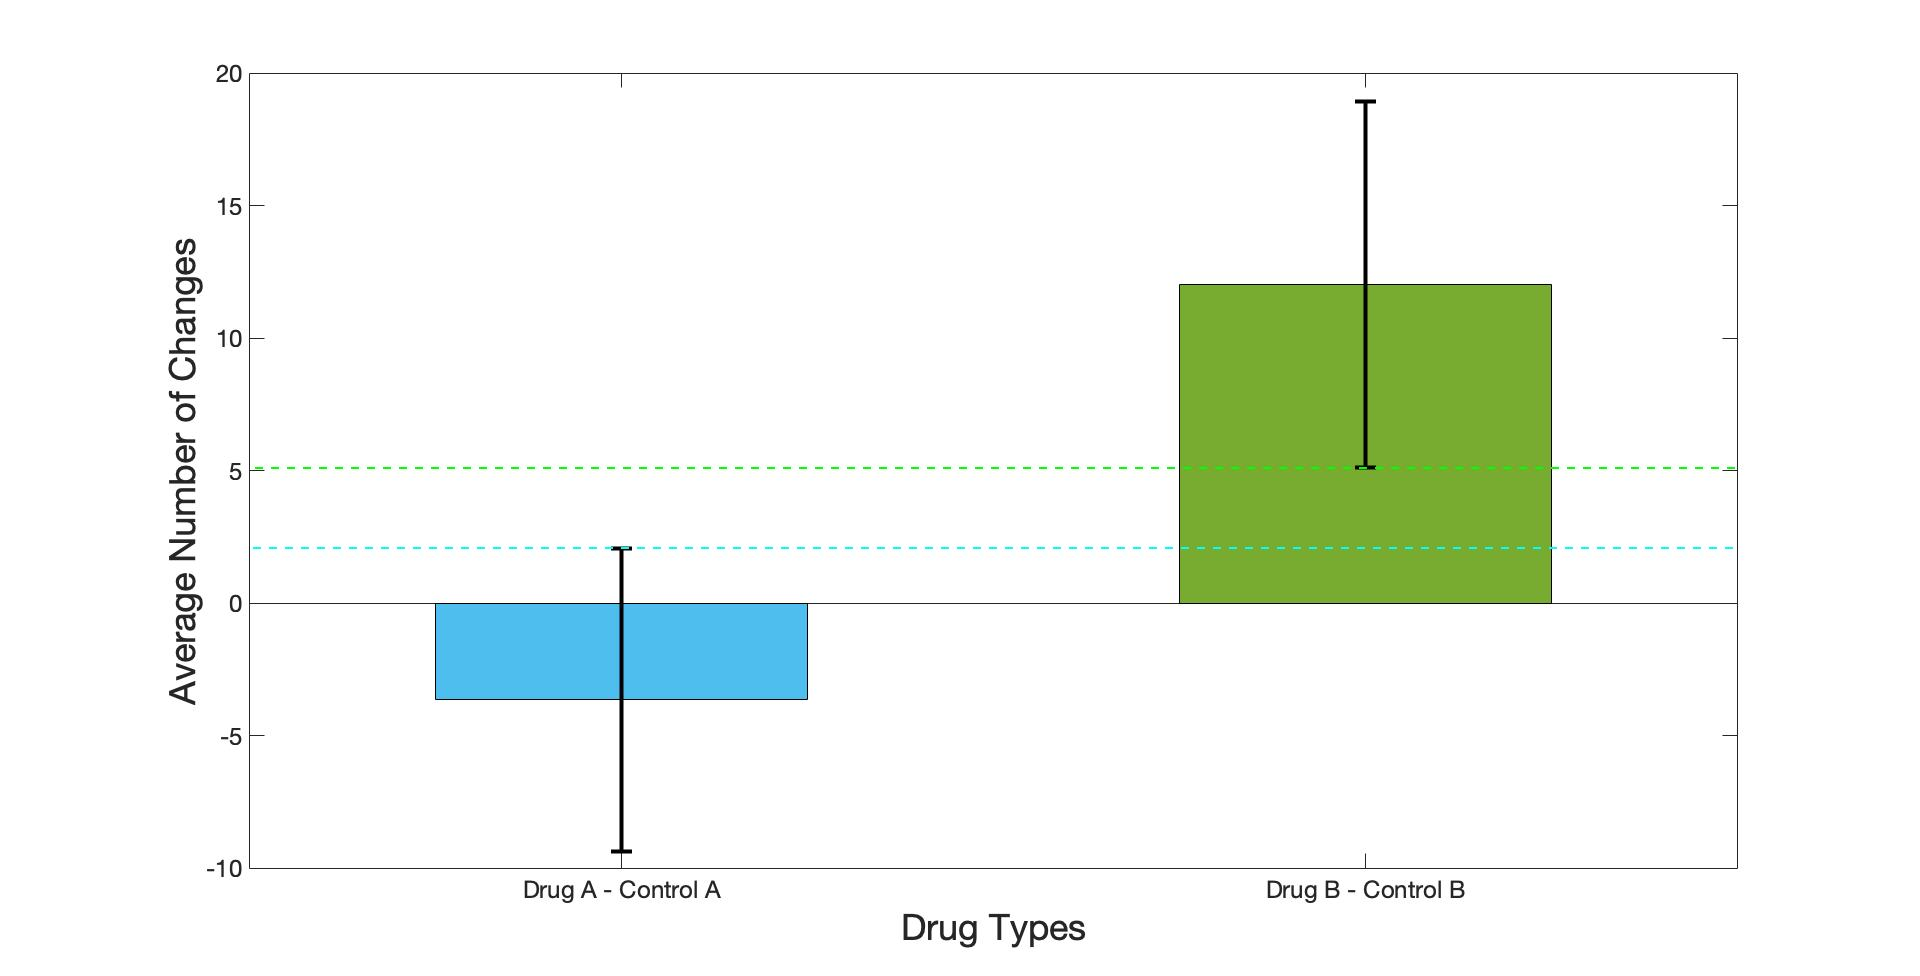
\includegraphics[width=\textwidth]{graph.jpg}
  \text{}\\
  \fbox{\begin{minipage}{53em}
    \begin{enumerate}
      \item What was your hypothesis?
      \item[-] My hypothesis on C. elegans on ethanol and caffeine would have a similar effect as humans would since we\\share a common ancestor. For humans, ethanol is a downer while caffeine is a upper. I would expect drug \DA{A}\\to be on the negative side of the graph and drug \DB{B} to be on the positive side of the graph with both drugs to\\have significant differences.
      \item Does the data support your hypothesis? In other words, what were the results of the experiment? Did Drug \DA{A}\\have a significant positive or negative effect? Did Drug \DB{B} have a significant positive or negative effect?
      \item[-] Drug \DA{A}'s confidence interval overlaps with zero, therefore ethanol has no significant difference on C. elegans.
      \item[-] Drug \DB{B}'s confidence interval do not overlap with zero, therefor caffeine has a significant difference on C. elegans.
      \item If the data does not show significance, why might this be?
      \item[-] Drug \DA{A} has no significant difference on C. elegans because
      \item Do you think it's an issue that Robyn knew which side of the slide was the control and which side contained\\the drug? Could this influence results?
      \item[-] d
    \end{enumerate}
  \end{minipage}}
\end{center}
\end{document}